\documentclass[12pt, a4paper]{article}

% ── Packages ──────────────────────────────────────────────────────────────────
\usepackage[utf8]{inputenc}
\usepackage[T1]{fontenc}

\usepackage[a4paper, margin=2.5cm, headheight=14pt]{geometry}
\usepackage{graphicx}
\usepackage{xcolor}
\usepackage{booktabs}
\usepackage{longtable}
\usepackage{array}
\usepackage{tabularx}
\usepackage{colortbl}
\usepackage{listings}
\usepackage{hyperref}
\usepackage{fancyhdr}
\usepackage{titlesec}
\usepackage{parskip}
\usepackage{enumitem}
\usepackage{caption}
\usepackage{float}


\usepackage{mdframed}
\usepackage{tocloft}
\usepackage{amssymb}

% ── Colors ────────────────────────────────────────────────────────────────────
\definecolor{teal}{HTML}{1A9E8F}
\definecolor{tealdark}{HTML}{0D7A6E}
\definecolor{teallight}{HTML}{E8F7F5}
\definecolor{tealmid}{HTML}{C5EBE6}
\definecolor{codebg}{HTML}{F4F4F4}
\definecolor{codefg}{HTML}{2D2D2D}
\definecolor{tableheader}{HTML}{1A9E8F}
\definecolor{tablerowalt}{HTML}{F5F5F5}
\definecolor{gray60}{HTML}{666666}
\definecolor{gray30}{HTML}{CCCCCC}
\definecolor{successgreen}{HTML}{16A34A}
\definecolor{warnyellow}{HTML}{D97706}
\definecolor{dangerred}{HTML}{DC2626}

% ── Hyperref ──────────────────────────────────────────────────────────────────
\hypersetup{
    colorlinks=true,
    linkcolor=teal,
    urlcolor=teal,
    citecolor=teal,
    pdftitle={RCP Data Imob - Documentação Completa},
    pdfauthor={Marcell Parra Araújo B. Silva, Rafael Vargas Carvalheira, Ruan Pablo Rodrigues}
}

% ── Section Titles ────────────────────────────────────────────────────────────
\titleformat{\section}
  {\Large\bfseries\color{teal}}
  {\thesection.}{0.5em}{}
  [\vspace{2pt}\color{teal}\titlerule\vspace{4pt}]

\titleformat{\subsection}
  {\large\bfseries\color{teal}}
  {\thesubsection}{0.5em}{}

\titleformat{\subsubsection}
  {\normalsize\bfseries}
  {\thesubsubsection}{0.5em}{}

\titlespacing{\section}{0pt}{18pt}{8pt}
\titlespacing{\subsection}{0pt}{12pt}{4pt}
\titlespacing{\subsubsection}{0pt}{8pt}{2pt}

% ── Header / Footer ───────────────────────────────────────────────────────────
\pagestyle{fancy}
\fancyhf{}
\fancyhead[L]{\small\color{gray60} RCP Data Imob — Documentação Completa}
\fancyhead[R]{\small\color{gray60} Lab. de Programação 3}
\fancyfoot[C]{\small\color{gray60}\thepage}
\renewcommand{\headrulewidth}{0.4pt}
\renewcommand{\headrule}{\hbox to\headwidth{\color{teal}\leaders\hrule height \headrulewidth\hfill}}

% ── Code Listings ─────────────────────────────────────────────────────────────
\lstset{
    backgroundcolor=\color{codebg},
    basicstyle=\ttfamily\small\color{codefg},
    breaklines=true,
    frame=single,
    framesep=4pt,
    rulecolor=\color{gray30},
    tabsize=2,
    showstringspaces=false,
    keywordstyle=\color{teal}\bfseries,
    stringstyle=\color{dangerred},
    commentstyle=\color{gray60}\itshape,
    numbers=none,
    xleftmargin=8pt,
    xrightmargin=8pt,
    aboveskip=8pt,
    belowskip=8pt,
}
\lstdefinelanguage{SQL2}{
    keywords={SELECT, FROM, WHERE, AND, OR, NOT, EXISTS, INSERT, UPDATE, DELETE, ALTER, TABLE, ADD, COLUMN, IF, SET, CASE, WHEN, THEN, ELSE, END, DEFAULT, IS, NULL},
    sensitive=false,
    morecomment=[l]{--},
    morestring=[b]',
}
\lstdefinelanguage{JavaScript2}{
    keywords={const, let, var, function, return, new, true, false, null, if, else, await},
    sensitive=true,
    morecomment=[l]{//},
    morestring=[b]",
    morestring=[b]',
}
\lstdefinelanguage{YAML2}{
    keywords={services, image, environment, ports, volumes, build, depends_on, condition},
    sensitive=false,
    morecomment=[l]{\#},
    morestring=[b]",
}

% ── Table helpers ─────────────────────────────────────────────────────────────
\newcommand{\thead}[1]{\cellcolor{tableheader}\color{white}\bfseries #1}
\newcommand{\talt}{\rowcolor{tablerowalt}}
\newcommand{\tok}{\textcolor{successgreen}{\textbf{Concluído}}}
\newcommand{\tstatus}[1]{\textcolor{teal}{\textbf{#1}}}

% ── Caption style ─────────────────────────────────────────────────────────────
\captionsetup{
    font=small,
    labelfont={bf,color=teal},
    textfont=it,
    justification=centering,
    skip=6pt
}

% ── TOC style ─────────────────────────────────────────────────────────────────
\renewcommand{\cftsecfont}{\bfseries\color{teal}}
\renewcommand{\cftsecpagefont}{\bfseries\color{teal}}
\renewcommand{\cftsubsecfont}{\color{teal}}
\setlength{\cftbeforesecskip}{4pt}

% ── Misc ──────────────────────────────────────────────────────────────────────
\setlength{\parindent}{0pt}
\setlength{\parskip}{6pt}
\graphicspath{{./}}

% ══════════════════════════════════════════════════════════════════════════════
\begin{document}

% ── Cover Page ────────────────────────────────────────────────────────────────
\begin{titlepage}
  \centering
  \vspace*{3cm}

  {\fontsize{36}{44}\selectfont\bfseries\color{teal} Sistema de Gestão de\\[6pt]}
  {\fontsize{36}{44}\selectfont\bfseries\color{black} Locações de Imóveis\\[20pt]}

  {\large\color{gray60} RCP Data Imob — Documentação Completa}

  \vspace{2cm}
  \color{gray30}\rule{0.6\textwidth}{0.4pt}\color{black}
  \vspace{1.5cm}

  {\normalsize Disciplina: \textbf{Laboratório de Programação 3}}\\[4pt]
  {\normalsize Professor: \textbf{Matheus Vanzan}}

  \vspace{1.5cm}

  {\normalsize\bfseries Integrantes:}\\[6pt]
  {\normalsize Marcell Parra Araújo B. Silva}\\[3pt]
  {\normalsize Rafael Vargas Carvalheira}\\[3pt]
  {\normalsize Ruan Pablo Rodrigues}

  \vspace{1.5cm}

  {\normalsize\color{teal} Março de 2026 — atualizado em Maio de 2026 (Entregável 8)}

  \vfill
  \color{gray30}\rule{0.6\textwidth}{0.4pt}
\end{titlepage}

% ── Table of Contents ─────────────────────────────────────────────────────────
\tableofcontents
\newpage

% ══════════════════════════════════════════════════════════════════════════════
\section{Apresentação do Projeto}

O projeto Sistema de Gestão de Locações de Imóveis consiste em uma aplicação web desenvolvida para apoiar a administração de imóveis destinados à locação. A proposta central do sistema é reunir, em uma única plataforma, as operações de cadastro de imóveis e clientes, controle de reservas, verificação de disponibilidade e acompanhamento financeiro da operação.

A solução foi concebida em arquitetura cliente-servidor desacoplada, com backend em API REST e frontend em SPA (Single Page Application). Essa separação facilita a manutenção do sistema, melhora a organização do código e permite reutilização futura da API por aplicações mobile.

Além disso, o projeto foi estruturado para atender aos requisitos práticos da disciplina, contemplando desde a definição do tema e da stack tecnológica até a implementação de serviços executáveis em ambiente containerizado e a disponibilização de endpoints REST organizados por entidade de negócio.

% ══════════════════════════════════════════════════════════════════════════════
\section{Objetivo do Sistema}

O objetivo do sistema é oferecer uma solução completa para o gerenciamento de locações de imóveis, permitindo:

\begin{itemize}[leftmargin=1.5em]
  \item Cadastrar e manter o portfólio de imóveis disponíveis;
  \item Cadastrar clientes e seus dados de contato;
  \item Criar, consultar, editar e cancelar locações;
  \item Verificar disponibilidade de imóveis com base em período e restrições de data;
  \item Categorizar imóveis por características relevantes;
  \item Registrar receitas e despesas associadas à operação;
  \item Acompanhar indicadores financeiros e operacionais.
\end{itemize}

Com isso, o sistema busca tornar o processo de administração de locações mais organizado, rastreável e eficiente.

% ══════════════════════════════════════════════════════════════════════════════
\section{Escopo Funcional}

O sistema foi planejado em torno de três módulos principais, detalhados a seguir.

\subsection{Gestão de Imóveis com Categorias}

Módulo responsável pelo cadastro e manutenção dos imóveis disponíveis para locação.

\begin{itemize}[leftmargin=1.5em]
  \item Cadastro completo de imóveis com informações como título, descrição, endereço, cidade, estado, CEP, número de quartos, banheiros, vagas de garagem, área, valor de aluguel e valor de venda;
  \item Associação de múltiplas categorias por imóvel (Piscina, Ar-condicionado, Pet-friendly, etc.);
  \item Criação de novas categorias durante o fluxo de cadastro;
  \item Busca e filtros por título, cidade e status de disponibilidade;
  \item Visualização em cards com informações resumidas;
  \item Edição e exclusão com validações de integridade.
\end{itemize}

\subsection{Sistema de Locações com Controle de Status}

Módulo central da aplicação, responsável pelo controle das locações.

\begin{itemize}[leftmargin=1.5em]
  \item Listagem de locações com imóvel, cliente, datas, valor mensal e status (ativa/inativa);
  \item Formulário de nova locação com selects dinâmicos de imóvel e cliente;
  \item Encerramento de locações ativas via PATCH;
  \item Indicação visual de locação ativa vs. inativa com badges semânticos;
  \item Cálculo e exibição de valor mensal em formato de moeda brasileira.
\end{itemize}

\subsection{Controle Financeiro com Dashboard Analítico}

Módulo que consolida receitas e despesas associadas à operação.

\begin{itemize}[leftmargin=1.5em]
  \item Registro de lançamentos financeiros com tipo (receita/despesa), valor, data de vencimento e locação associada;
  \item Filtros por status (pendente/pago/atrasado);
  \item Cards de resumo com total de receitas e total de despesas;
  \item Registro de pagamento via PATCH;
  \item Dashboard com KPIs consolidados e gráfico de evolução financeira dos últimos 6 meses;
  \item Listagem das últimas locações registradas.
\end{itemize}

% ══════════════════════════════════════════════════════════════════════════════
\section{Funcionalidade Selecionada para o Mobile}

A funcionalidade escolhida para adaptação em ambiente mobile foi a Busca de Disponibilidade e Criação de Reserva. Essa escolha foi motivada por se tratar de um fluxo frequente para administradores de imóveis, especialmente em situações fora do escritório.

Recursos previstos para o mobile:

\begin{itemize}[leftmargin=1.5em]
  \item Tela com campos de data de entrada e saída para busca rápida;
  \item Listagem de imóveis disponíveis no período informado;
  \item Exibição resumida com tipo, capacidade e valor estimado;
  \item Tela de detalhes do imóvel com categorias;
  \item Confirmação de reserva com seleção de cliente;
  \item Feedback imediato em caso de sucesso ou conflito de datas.
\end{itemize}

\textbf{Justificativa:} A consulta de disponibilidade e a confirmação de reservas são tarefas que exigem agilidade. Uma versão mobile desse fluxo reduz a dependência de computador e acelera o atendimento ao cliente.

% ══════════════════════════════════════════════════════════════════════════════
\section{Arquitetura da Solução}

A aplicação adota uma arquitetura dividida em três camadas principais:

\begin{itemize}[leftmargin=1.5em]
  \item \textbf{Banco de dados:} responsável pelo armazenamento persistente dos dados do sistema;
  \item \textbf{Backend:} responsável pela lógica de negócio, exposição dos endpoints e comunicação com o banco;
  \item \textbf{Frontend:} responsável pela interface visual e interação com o usuário.
\end{itemize}

Os serviços são orquestrados com Docker Compose, o que simplifica a execução do ambiente de desenvolvimento e padroniza a configuração entre diferentes máquinas.

\subsection{Serviços e Portas}

\begin{table}[H]
\centering
\begin{tabularx}{\textwidth}{|l|l|l|X|}
\hline
\thead{Serviço} & \thead{Imagem / Tecnologia} & \thead{Porta} & \thead{Descrição} \\
\hline
db       & postgres:13-alpine      & 5432 & Banco de dados PostgreSQL \\
\talt backend  & node:18-alpine (build)  & 3000 & API REST Node.js / Express \\
frontend & node:20-alpine (build)  & 5173 & Interface React / Vite \\
\hline
\end{tabularx}
\caption{Serviços e portas do ambiente Docker}
\end{table}

% ══════════════════════════════════════════════════════════════════════════════
\section{Stack Tecnológica}

\subsection{Backend}

\begin{table}[H]
\centering
\begin{tabularx}{\textwidth}{|l|l|X|}
\hline
\thead{Tecnologia} & \thead{Versão} & \thead{Função no projeto} \\
\hline
Node.js      & v18+   & Runtime JavaScript no servidor \\
\talt Express.js  & 4.18.2 & Framework para API REST \\
PostgreSQL   & v13+   & Banco de dados relacional principal \\
\talt pg           & 8.11.3 & Driver PostgreSQL para Node.js \\
cors         & 2.8.5  & Middleware para Cross-Origin Requests \\
\hline
\end{tabularx}
\caption{Stack do backend}
\end{table}

\subsection{Frontend}

\begin{table}[H]
\centering
\begin{tabularx}{\textwidth}{|l|l|X|}
\hline
\thead{Tecnologia} & \thead{Versão} & \thead{Função no projeto} \\
\hline
React           & v18.2  & Construção da interface SPA \\
\talt Vite           & v6.0   & Build tool e servidor de desenvolvimento \\
React Router DOM & v7.0  & Roteamento client-side \\
\talt Tailwind CSS  & v3.4   & Estilização responsiva com utility-first \\
Recharts        & v2.12  & Gráficos do dashboard financeiro \\
\talt Lucide React  & v0.400 & Biblioteca de ícones \\
Axios           & v1.7   & Comunicação HTTP com a API \\
\hline
\end{tabularx}
\caption{Stack do frontend}
\end{table}

\subsection{Mobile}

\begin{table}[H]
\centering
\begin{tabularx}{\textwidth}{|l|l|X|}
\hline
\thead{Tecnologia} & \thead{Versão} & \thead{Função no projeto} \\
\hline
React Native & 0.81 & Construção da interface mobile nativa \\
\talt Expo & SDK 54 & Execução local, Metro Bundler e suporte ao Expo Go \\
React Navigation & 7.x & Navegação por abas e pilha de telas \\
\talt Expo Vector Icons & 15.x & Ícones da interface mobile \\
Fetch API & Nativo & Comunicação HTTP com a API REST existente \\
\hline
\end{tabularx}
\caption{Stack do MVP mobile}
\end{table}

\subsection{Infraestrutura}

\begin{table}[H]
\centering
\begin{tabularx}{\textwidth}{|l|X|}
\hline
\thead{Tecnologia} & \thead{Função} \\
\hline
Docker         & Containerização dos serviços \\
\talt Docker Compose & Orquestração multi-container \\
Google Fonts   & Tipografia (Plus Jakarta Sans + DM Sans) \\
\hline
\end{tabularx}
\caption{Infraestrutura}
\end{table}

% ══════════════════════════════════════════════════════════════════════════════
\section{Modelo de Dados}

As tabelas principais do sistema estão organizadas conforme a estrutura abaixo.

\begin{table}[H]
\centering
\begin{tabularx}{\textwidth}{|l|X|}
\hline
\thead{Tabela} & \thead{Conteúdo} \\
\hline
usuarios            & Dados de acesso e perfil dos administradores \\
\talt imoveis            & Cadastro dos imóveis com atributos, valores e status \\
categorias\_imoveis & Categorias personalizadas para classificação \\
\talt imovel\_categorias & Relacionamento N:N entre imóveis e categorias \\
clientes            & Cadastro de locatários \\
\talt locacoes           & Contratos de locação, datas, valores e status \\
financeiro          & Lançamentos de receitas e despesas \\
\hline
\end{tabularx}
\caption{Tabelas do sistema}
\end{table}

\subsection{Diagrama de Relacionamentos}

\begin{lstlisting}
categorias_imoveis --(N:N)-- imovel_categorias --(N:N)-- imoveis
                                                              |
                                                           (1:N)
                                                              |
                       locacoes --(1:N)-- financeiro       imoveis
                           |
                         (N:1)
                           |
                        clientes
\end{lstlisting}

\subsection{Detalhamento das Tabelas}

\subsubsection{Tabela: imoveis}

\begin{table}[H]
\centering
\begin{tabularx}{\textwidth}{|l|l|l|X|}
\hline
\thead{Coluna} & \thead{Tipo} & \thead{Restrições} & \thead{Descrição} \\
\hline
id             & SERIAL         & PRIMARY KEY  & Identificador único \\
\talt titulo        & VARCHAR(255)   & NOT NULL     & Título do imóvel \\
descricao      & TEXT           & —            & Descrição detalhada \\
\talt endereco      & VARCHAR(500)   & NOT NULL     & Endereço completo \\
cidade         & VARCHAR(100)   & —            & Cidade \\
\talt estado        & VARCHAR(2)     & —            & UF \\
cep            & VARCHAR(10)    & —            & CEP \\
\talt valor\_aluguel & NUMERIC(12,2) & —           & Valor mensal de aluguel \\
valor\_venda   & NUMERIC(12,2)  & —            & Valor de venda \\
\talt area          & NUMERIC(10,2)  & —            & Área em m² \\
quartos        & INTEGER        & DEFAULT 0    & Número de quartos \\
\talt banheiros     & INTEGER        & DEFAULT 0    & Número de banheiros \\
vagas\_garagem & INTEGER        & DEFAULT 0    & Vagas de garagem \\
\talt disponivel    & BOOLEAN        & DEFAULT TRUE & Disponível para locação \\
criado\_em     & TIMESTAMP      & DEFAULT NOW()& Data de cadastro \\
\hline
\end{tabularx}
\caption{Estrutura da tabela imoveis}
\end{table}

\subsubsection{Tabela: clientes}

\begin{table}[H]
\centering
\begin{tabularx}{\textwidth}{|l|l|l|X|}
\hline
\thead{Coluna} & \thead{Tipo} & \thead{Restrições} & \thead{Descrição} \\
\hline
id         & SERIAL       & PRIMARY KEY   & Identificador único \\
\talt nome      & VARCHAR(255) & NOT NULL      & Nome completo \\
cpf        & VARCHAR(14)  & UNIQUE        & CPF (000.000.000-00) \\
\talt email     & VARCHAR(255) & —             & E-mail de contato \\
telefone   & VARCHAR(20)  & —             & Telefone \\
\talt endereco  & VARCHAR(500) & —             & Endereço do cliente \\
criado\_em & TIMESTAMP    & DEFAULT NOW() & Data de cadastro \\
\hline
\end{tabularx}
\caption{Estrutura da tabela clientes}
\end{table}

\subsubsection{Tabela: locacoes}

\begin{table}[H]
\centering
\begin{tabularx}{\textwidth}{|l|l|l|X|}
\hline
\thead{Coluna} & \thead{Tipo} & \thead{Restrições} & \thead{Descrição} \\
\hline
id           & SERIAL        & PRIMARY KEY        & Identificador único \\
\talt imovel\_id  & INTEGER       & FK → imoveis(id)   & Imóvel locado \\
cliente\_id  & INTEGER       & FK → clientes(id)  & Locatário \\
\talt data\_inicio & DATE          & NOT NULL           & Início do contrato \\
data\_fim    & DATE          & —                  & Fim do contrato \\
\talt valor\_mensal& NUMERIC(12,2) & NOT NULL           & Valor mensal \\
status       & VARCHAR(50)   & DEFAULT 'pendente' & pendente | confirmada | cancelada \\
\talt valor\_total & NUMERIC(12,2) & —                  & Valor total calculado \\
ativa        & BOOLEAN       & DEFAULT TRUE       & Locação em vigor \\
\talt criado\_em   & TIMESTAMP     & DEFAULT NOW()      & Data de registro \\
\hline
\end{tabularx}
\caption{Estrutura da tabela locacoes}
\end{table}

\subsubsection{Tabela: financeiro}

\begin{table}[H]
\centering
\begin{tabularx}{\textwidth}{|l|l|l|X|}
\hline
\thead{Coluna} & \thead{Tipo} & \thead{Restrições} & \thead{Descrição} \\
\hline
id               & SERIAL        & PRIMARY KEY          & Identificador único \\
\talt locacao\_id     & INTEGER       & FK → locacoes(id)    & Locação relacionada \\
tipo             & VARCHAR(50)   & NOT NULL             & receita / despesa \\
\talt valor           & NUMERIC(12,2) & NOT NULL             & Valor do lançamento \\
data\_vencimento & DATE          & NOT NULL             & Data de vencimento \\
\talt data\_pagamento & DATE          & —                    & Data de pagamento \\
status           & VARCHAR(50)   & DEFAULT 'pendente'   & pendente / pago / atrasado \\
\talt criado\_em      & TIMESTAMP     & DEFAULT NOW()        & Data de registro \\
\hline
\end{tabularx}
\caption{Estrutura da tabela financeiro}
\end{table}

% ══════════════════════════════════════════════════════════════════════════════
\section{Estrutura do Backend}

O backend foi organizado de forma modular, com separação entre ponto de entrada, acesso ao banco e rotas por entidade.

\subsection{Organização do Projeto}

\begin{table}[H]
\centering
\begin{tabularx}{\textwidth}{|l|X|}
\hline
\thead{Caminho} & \thead{Descrição} \\
\hline
backend/src/index.js            & Ponto de entrada; inicializa o Express e registra as rotas \\
\talt backend/src/db/pool.js         & Pool de conexão com PostgreSQL \\
backend/src/routes/imoveis.js   & Rotas CRUD de imóveis + disponibilidade (F1) \\
\talt backend/src/routes/clientes.js & Rotas CRUD de clientes \\
backend/src/routes/locacoes.js  & Rotas CRUD de locações \\
\talt backend/src/routes/categorias.js & Rotas CRUD de categorias \\
backend/src/routes/financeiro.js & Rotas CRUD de lançamentos financeiros \\
\talt backend/src/routes/status.js   & Endpoint de healthcheck \\
\hline
\end{tabularx}
\caption{Organização dos arquivos do backend}
\end{table}

\subsection{Conexão com o Banco de Dados}

A comunicação com o PostgreSQL é realizada por meio de um pool de conexões (\texttt{pg.Pool}). Esse mecanismo evita a abertura e o fechamento de uma nova conexão a cada requisição, reduzindo overhead e melhorando a eficiência do backend.

\begin{lstlisting}[language=JavaScript2]
const pool = new Pool({
  host: process.env.DB_HOST || 'localhost',
  port: process.env.DB_PORT || 5432,
  database: process.env.DB_NAME || 'rcp_data_imob',
  user: process.env.DB_USER || 'admin',
  password: process.env.DB_PASSWORD || 'admin123',
});
\end{lstlisting}

\subsection{Variáveis de Ambiente}

\begin{table}[H]
\centering
\begin{tabularx}{\textwidth}{|l|l|X|}
\hline
\thead{Variável} & \thead{Valor padrão} & \thead{Descrição} \\
\hline
DB\_HOST     & db            & Host do serviço PostgreSQL no Compose \\
\talt DB\_PORT     & 5432          & Porta do PostgreSQL \\
DB\_NAME     & rcp\_data\_imob & Nome do banco de dados \\
\talt DB\_USER     & admin         & Usuário de acesso \\
DB\_PASSWORD & admin123      & Senha de acesso \\
\hline
\end{tabularx}
\caption{Variáveis de ambiente do backend}
\end{table}

% ══════════════════════════════════════════════════════════════════════════════
\section{API REST}

A API foi construída com Node.js e Express, seguindo princípios REST para organização de recursos, uso semântico dos verbos HTTP e respostas padronizadas em JSON. O servidor escuta na porta 3000, e as rotas estão separadas por entidade.

\subsection{Endpoint de Healthcheck}

\begin{table}[H]
\centering
\begin{tabularx}{\textwidth}{|l|l|l|X|}
\hline
\thead{Método} & \thead{Rota} & \thead{Descrição} & \thead{Resposta} \\
\hline
GET & /status & Verifica status da aplicação e do banco & \texttt{\{"status":"ok","banco":"conectado"\}} \\
\hline
\end{tabularx}
\end{table}

\subsection{Endpoints de Imóveis}

\begin{table}[H]
\centering
\begin{tabularx}{\textwidth}{|l|l|X|}
\hline
\thead{Método} & \thead{Rota} & \thead{Descrição} \\
\hline
GET    & /imoveis                   & Lista todos os imóveis cadastrados \\
\talt GET    & /imoveis/disponibilidade   & Lista imóveis livres em período (F1) com categorias \\
GET    & /imoveis/:id               & Retorna um imóvel específico pelo ID \\
\talt POST   & /imoveis                   & Cria um novo imóvel \\
PUT    & /imoveis/:id               & Atualiza os dados de um imóvel \\
\talt DELETE & /imoveis/:id               & Remove um imóvel do sistema \\
\hline
\end{tabularx}
\caption{Endpoints de imóveis}
\end{table}

\subsection{Endpoints de Clientes}

\begin{table}[H]
\centering
\begin{tabularx}{\textwidth}{|l|l|X|}
\hline
\thead{Método} & \thead{Rota} & \thead{Descrição} \\
\hline
GET    & /clientes     & Lista todos os clientes cadastrados \\
\talt GET    & /clientes/:id & Retorna um cliente específico pelo ID \\
POST   & /clientes     & Cadastra um novo cliente \\
\talt PUT    & /clientes/:id & Atualiza os dados de um cliente \\
DELETE & /clientes/:id & Remove um cliente do sistema \\
\hline
\end{tabularx}
\caption{Endpoints de clientes}
\end{table}

\subsection{Endpoints de Locações}

\begin{table}[H]
\centering
\begin{tabularx}{\textwidth}{|l|l|X|}
\hline
\thead{Método} & \thead{Rota} & \thead{Descrição} \\
\hline
GET   & /locacoes                 & Lista todas as locações (aceita \texttt{?status=}) \\
\talt GET   & /locacoes/:id             & Retorna uma locação específica \\
POST  & /locacoes                 & Cria um novo contrato de locação \\
\talt PUT   & /locacoes/:id             & Edição completa com revalidação de disponibilidade \\
PATCH & /locacoes/:id/status      & Altera apenas o status, revalidando conflito ao confirmar \\
\talt PATCH & /locacoes/:id/encerrar    & Encerra uma locação ativa (status=cancelada) \\
\hline
\end{tabularx}
\caption{Endpoints de locações}
\end{table}

\subsection{Endpoints de Categorias}

\begin{table}[H]
\centering
\begin{tabularx}{\textwidth}{|l|l|X|}
\hline
\thead{Método} & \thead{Rota} & \thead{Descrição} \\
\hline
GET    & /categorias     & Lista todas as categorias disponíveis \\
\talt POST   & /categorias     & Cria uma nova categoria \\
DELETE & /categorias/:id & Remove uma categoria do sistema \\
\hline
\end{tabularx}
\caption{Endpoints de categorias}
\end{table}

\subsection{Endpoints Financeiros}

\begin{table}[H]
\centering
\begin{tabularx}{\textwidth}{|l|l|X|}
\hline
\thead{Método} & \thead{Rota} & \thead{Descrição} \\
\hline
GET    & /financeiro            & Lista lançamentos com filtros (\texttt{?tipo=\&status=\&locacao\_id=\&data\_inicio=\&data\_fim=}) \\
\talt GET    & /financeiro/resumo     & KPIs analíticos: receitas, despesas, saldo, pendentes, atrasados (F3) \\
GET    & /financeiro/por-mes    & Série temporal agregada (\texttt{?meses=N}) para gráficos (F3) \\
\talt GET    & /financeiro/:id        & Detalhe de um lançamento por ID (F3) \\
POST   & /financeiro            & Registra um novo lançamento (aceita \texttt{descricao}) \\
\talt PUT    & /financeiro/:id        & Edição completa do lançamento (F3) \\
PATCH  & /financeiro/:id/pagar  & Registra pagamento de um lançamento \\
\talt DELETE & /financeiro/:id        & Remove o lançamento (F3) \\
\hline
\end{tabularx}
\caption{Endpoints financeiros (atualizados pela F3)}
\end{table}

\subsection{Resumo Geral dos Endpoints}

\begin{table}[H]
\centering
\begin{tabular}{|l|c|c|c|c|c|c|}
\hline
\thead{Entidade} & \thead{GET} & \thead{POST} & \thead{PUT} & \thead{PATCH} & \thead{DELETE} & \thead{Total} \\
\hline
/status      & 1  & —  & —  & —  & —  & 1  \\
\talt /imoveis     & 3  & 1  & 1  & —  & 1  & 6  \\
/clientes    & 2  & 1  & 1  & —  & 1  & 5  \\
\talt /locacoes    & 2  & 1  & 1  & 2  & —  & 6  \\
/categorias  & 1  & 1  & —  & —  & 1  & 3  \\
\talt /financeiro  & 4  & 1  & 1  & 1  & 1  & 8  \\
\hline
\textbf{TOTAL} & \textbf{13} & \textbf{5} & \textbf{4} & \textbf{3} & \textbf{4} & \textbf{29} \\
\hline
\end{tabular}
\caption{Resumo geral dos endpoints da API}
\end{table}

% ══════════════════════════════════════════════════════════════════════════════
\section{Banco de Dados e Docker (Entregável 3)}

O Entregável 3 consolidou a configuração do banco de dados PostgreSQL via Docker, a modelagem das entidades do sistema e a integração completa entre o backend Node.js/Express e o banco de dados. O ambiente é orquestrado pelo Docker Compose, garantindo portabilidade e facilidade de execução em qualquer máquina.

\subsection{Status dos Requisitos}

\begin{table}[H]
\centering
\begin{tabularx}{\textwidth}{|X|l|}
\hline
\thead{Requisito} & \thead{Status} \\
\hline
Banco de dados configurado no Docker (PostgreSQL 13) & \tok \\
\talt Modelagem das entidades e relacionamentos & \tok \\
Backend integrado ao banco com persistência via API & \tok \\
\talt CRUD completo testado via Postman & \tok \\
Documentação e capturas de tela & \tok \\
\hline
\end{tabularx}
\caption{Status dos requisitos — Entregável 3}
\end{table}

\subsection{Configuração do docker-compose.yml}

\begin{lstlisting}[language=YAML2]
services:
  db:
    image: postgres:13-alpine
    environment:
      POSTGRES_DB: rcp_data_imob
      POSTGRES_USER: admin
      POSTGRES_PASSWORD: admin123
    ports:
      - "5432:5432"
    volumes:
      - pgdata:/var/lib/postgresql/data
      - ./database/init.sql:/docker-entrypoint-initdb.d/init.sql
  backend:
    build: ./backend
    ports:
      - "3000:3000"
    environment:
      DB_HOST: db
      DB_PORT: 5432
      DB_NAME: rcp_data_imob
      DB_USER: admin
      DB_PASSWORD: admin123
  frontend:
    build: ./frontend
    ports:
      - "5173:5173"
    environment:
      - VITE_API_URL=http://localhost:3000
volumes:
  pgdata:
\end{lstlisting}

\subsection{Testes CRUD via Postman}

\begin{table}[H]
\centering
\begin{tabular}{|l|l|l|l|}
\hline
\thead{Operação} & \thead{Método} & \thead{Endpoint} & \thead{Status} \\
\hline
Create       & POST   & /clientes     & 201 Created \\
\talt Read (listar) & GET    & /clientes     & 200 OK \\
Update       & PUT    & /clientes/:id & 200 OK \\
\talt Delete       & DELETE & /clientes/:id & 200 OK \\
\hline
\end{tabular}
\caption{Testes CRUD via Postman}
\end{table}

% ══════════════════════════════════════════════════════════════════════════════
\section{Frontend e Docker (Entregável 4)}

O Entregável 4 implementou o frontend completo do sistema com React, configurado e executável via Docker, consumindo dados reais da API REST do backend.

\subsection{Requisitos Atendidos}

\begin{table}[H]
\centering
\begin{tabularx}{\textwidth}{|X|l|}
\hline
\thead{Requisito} & \thead{Status} \\
\hline
Frontend configurado e rodando no Docker & \tok \\
\talt Tela inicial do sistema criada (Dashboard) & \tok \\
Navegação mínima entre telas (menu/rotas) & \tok \\
\talt Frontend consumindo dados da API (múltiplas chamadas) & \tok \\
Exibição de dados vindos da API (listas, KPIs, gráficos) & \tok \\
\talt Documentação correspondente e capturas de tela & \tok \\
\hline
\end{tabularx}
\caption{Status dos requisitos — Entregável 4}
\end{table}

\subsection{Telas Implementadas}

\begin{table}[H]
\centering
\begin{tabularx}{\textwidth}{|l|l|X|}
\hline
\thead{Rota} & \thead{Tela} & \thead{Funcionalidades} \\
\hline
/           & Dashboard  & 4 KPIs, gráfico de barras (Recharts) com 6 meses, últimas locações \\
\talt /imoveis    & Imóveis    & Cards com filtros (cidade/status/busca), CRUD completo via modal \\
/clientes   & Clientes   & Tabela com busca por nome, CRUD completo via modal \\
\talt /locacoes   & Locações   & Tabela com selects de imóvel/cliente, encerramento de locação \\
/financeiro & Financeiro & Cards receitas/despesas, filtro por status, ação de pagamento \\
\hline
\end{tabularx}
\caption{Telas implementadas no frontend}
\end{table}

\subsection{Consumo da API}

\begin{table}[H]
\centering
\begin{tabularx}{\textwidth}{|l|X|}
\hline
\thead{Tela} & \thead{Endpoints consumidos} \\
\hline
Dashboard   & GET /imoveis, GET /clientes, GET /locacoes, GET /financeiro \\
\talt Imóveis    & GET /imoveis, POST /imoveis, PUT /imoveis/:id, DELETE /imoveis/:id \\
Clientes    & GET /clientes, POST /clientes, PUT /clientes/:id, DELETE /clientes/:id \\
\talt Locações   & GET /locacoes, GET /imoveis, GET /clientes, POST /locacoes, PATCH /locacoes/:id/encerrar \\
Financeiro  & GET /financeiro, GET /locacoes, POST /financeiro, PATCH /financeiro/:id/pagar \\
\hline
\end{tabularx}
\caption{Consumo da API por tela}
\end{table}

% ══════════════════════════════════════════════════════════════════════════════
\section{Capturas de Tela do Frontend (Entregável 4)}

A seguir são apresentadas as capturas de tela das 5 telas principais do sistema, documentando o estado visual de cada módulo implementado.

\subsection{Dashboard}

Tela inicial com visão geral do sistema: 4 cards de KPIs (Total de Imóveis, Total de Clientes, Locações Ativas, Receita do Mês), gráfico de evolução financeira dos últimos 6 meses (Recharts) e lista das últimas locações.

\begin{figure}[H]
  \centering
  
\includegraphics[width=\textwidth]{tela-dashboard.png}
  \caption{Dashboard com KPIs, gráfico de evolução financeira e últimas locações}
  \label{fig:dashboard}
\end{figure}

\subsection{Imóveis}

Tela de gestão de imóveis com barra de busca por título, filtros por cidade e status de disponibilidade, e botão ``Novo Imóvel'' para cadastro. Os imóveis são exibidos em cards com informações resumidas.

\begin{figure}[H]
  \centering
  
\includegraphics[width=\textwidth]{tela-imoveis.png}
  \caption{Listagem de imóveis com filtros e busca}
  \label{fig:imoveis}
\end{figure}

\subsection{Clientes}

Tela de gestão de clientes com busca por nome e botão ``Novo Cliente''. Os dados são apresentados em tabela com colunas Nome, CPF, Email, Telefone e ações de edição/exclusão.

\begin{figure}[H]
  \centering
  
\includegraphics[width=\textwidth]{tela-clientes.png}
  \caption{Listagem de clientes com busca por nome}
  \label{fig:clientes}
\end{figure}

\subsection{Locações}

Tela de gestão de locações com listagem de contratos contendo imóvel, cliente, datas, valor mensal e status (ativo/inativo). Botão ``Nova Locação'' para registro com selects dinâmicos.

\begin{figure}[H]
  \centering
  
\includegraphics[width=\textwidth]{tela-locacoes.png}
  \caption{Listagem de locações com status e ação de encerramento}
  \label{fig:locacoes}
\end{figure}

\subsection{Financeiro}

Tela financeira com cards de resumo (Total Receitas e Total Despesas), filtro por status (pendente/pago/atrasado), e tabela de lançamentos com ação de pagamento.

\begin{figure}[H]
  \centering
  
\includegraphics[width=\textwidth]{tela-financeiro.png}
  \caption{Painel financeiro com resumo e filtros por status}
  \label{fig:financeiro}
\end{figure}

% ══════════════════════════════════════════════════════════════════════════════
\section{Funcionalidade F1 — Busca de Disponibilidade e Criação de Reserva (Entregável 5)}

\subsection{Descrição}

O Entregável 5 implementou a Funcionalidade F1 completa: Busca de Disponibilidade e Criação de Reserva. Esta funcionalidade permite ao usuário buscar imóveis disponíveis em um período específico e criar reservas diretamente pela interface web.

\subsection{Requisitos Atendidos}

\begin{table}[H]
\centering
\begin{tabularx}{\textwidth}{|X|l|}
\hline
\thead{Requisito} & \thead{Status} \\
\hline
Endpoint da API para busca de disponibilidade implementado & \tok \\
\talt Lógica de conflito de datas no banco & \tok \\
Retorno de categorias do imóvel no endpoint & \tok \\
\talt Tela de busca com campos de período & \tok \\
Listagem de imóveis disponíveis em cards & \tok \\
\talt Modal de confirmação de reserva com seleção de cliente & \tok \\
Feedback de sucesso e atualização da listagem & \tok \\
\talt Fluxo completo funcionando no Docker & \tok \\
\hline
\end{tabularx}
\caption{Status dos requisitos — Entregável 5 (F1)}
\end{table}

\subsection{Endpoint Implementado}

\begin{table}[H]
\centering
\begin{tabularx}{\textwidth}{|l|l|l|X|}
\hline
\thead{Método} & \thead{Rota} & \thead{Parâmetros} & \thead{Descrição} \\
\hline
GET & /imoveis/disponibilidade & data\_inicio, data\_fim (query) & Lista imóveis disponíveis no período com categorias \\
\hline
\end{tabularx}
\end{table}

Lógica de conflito de datas: um imóvel é considerado \textbf{INDISPONÍVEL} se existir uma locação ativa (\texttt{ativa = true}) cujo período se sobreponha ao período solicitado:

\begin{lstlisting}[language=SQL2]
NOT EXISTS (
  SELECT 1 FROM locacoes l
  WHERE l.imovel_id = i.id
    AND l.ativa = true
    AND l.data_inicio <= data_fim
    AND (l.data_fim IS NULL OR l.data_fim >= data_inicio)
)
\end{lstlisting}

Isso garante que:
\begin{itemize}[leftmargin=1.5em]
  \item Locações sem \texttt{data\_fim} (abertas) bloqueiam o imóvel indefinidamente;
  \item Qualquer sobreposição parcial de período também bloqueia;
  \item Apenas locações ativas (\texttt{ativa = true}) são consideradas no bloqueio.
\end{itemize}

\subsection{Fluxo Completo da F1}

\begin{enumerate}[leftmargin=1.5em]
  \item O usuário acessa a tela ``Disponibilidade'' via sidebar (ícone CalendarSearch);
  \item Preenche Data de Entrada e Data de Saída e clica em ``Buscar Disponíveis'';
  \item O frontend chama \texttt{GET /imoveis/disponibilidade?data\_inicio=\&data\_fim=};
  \item Imóveis disponíveis são exibidos em cards com: título, cidade/estado, quartos, banheiros, vagas de garagem, área, categorias como badges coloridos e valor mensal;
  \item O usuário clica em ``Reservar'' em um imóvel;
  \item Modal de confirmação é exibido com: resumo do imóvel, período pré-preenchido (readonly), select de cliente, campo de valor mensal editável;
  \item Ao confirmar, o frontend chama \texttt{POST /locacoes} criando a locação no banco;
  \item Banner de sucesso é exibido e o imóvel é removido da listagem;
  \item Em caso de erro (ex: conflito), mensagem de erro aparece no modal.
\end{enumerate}

\subsection{Arquivos Criados/Modificados}

\begin{table}[H]
\centering
\begin{tabularx}{\textwidth}{|l|l|X|}
\hline
\thead{Arquivo} & \thead{Operação} & \thead{Descrição} \\
\hline
backend/src/routes/imoveis.js           & Modificado & Adicionado endpoint GET /disponibilidade com lógica SQL de conflito \\
\talt frontend/src/pages/Disponibilidade.jsx & Criado     & Nova página com form de busca, cards e modal de reserva \\
frontend/src/App.jsx                    & Modificado & Rota /disponibilidade adicionada \\
\talt frontend/src/components/Layout.jsx    & Modificado & Item ``Disponibilidade'' com ícone CalendarSearch na sidebar \\
\hline
\end{tabularx}
\caption{Arquivos criados/modificados — Entregável 5}
\end{table}

\subsection{Testes Realizados}

\begin{table}[H]
\centering
\begin{tabularx}{\textwidth}{|X|l|l|}
\hline
\thead{Teste} & \thead{Esperado} & \thead{Resultado} \\
\hline
GET /disponibilidade sem params          & HTTP 400              & Passou \\
\talt Busca em período livre (2 imóveis disponíveis) & 2 imóveis   & Passou \\
Busca em período com imóvel ocupado     & 1 imóvel (conflito)   & Passou \\
\talt Categorias retornadas no JSON          & Array categorias      & Passou \\
Criar reserva via POST /locacoes        & Locação criada ativa=true & Passou \\
\talt Busca após reserva (imóvel some)       & 1 imóvel removido     & Passou \\
Endpoint via proxy Vite /api/...        & JSON com categorias   & Passou \\
\talt Frontend acessível em localhost:5173   & HTTP 200              & Passou \\
\hline
\end{tabularx}
\caption{Testes realizados — Entregável 5}
\end{table}

% ══════════════════════════════════════════════════════════════════════════════
\section{Funcionalidade F2 — Sistema de Reservas com Status (Entregável 6)}

\subsection{Visão Geral}

O Entregável 6 implementa a Funcionalidade F2 — Sistema de Reservas com Verificação de Disponibilidade, expandindo o módulo de locações com controle completo de ciclo de vida de reservas. As principais adições são: campo \texttt{status} (Pendente / Confirmada / Cancelada) na tabela de locações, cálculo automático de valor total, edição de reservas existentes com revalidação de conflito de datas, e tela de Agenda com calendário mensal interativo.

\begin{table}[H]
\centering
\begin{tabularx}{\textwidth}{|X|l|}
\hline
\thead{Requisito} & \thead{Status} \\
\hline
Status de reserva (Pendente / Confirmada / Cancelada) no banco e na API & \tok \\
\talt Edição de reservas com revalidação de disponibilidade & \tok \\
Cálculo automático de valor total com base no período & \tok \\
\talt Tela de Agenda — calendário mensal com cores por status & \tok \\
Filtros por status na listagem de locações & \tok \\
\talt Fluxo completo funcionando no Docker & \tok \\
\hline
\end{tabularx}
\caption{Status dos requisitos — Entregável 6 (F2)}
\end{table}

\subsection{Alterações no Banco de Dados}

\subsubsection{Migração aplicada à tabela locacoes}

Foram adicionadas duas novas colunas à tabela existente via script de migração (\texttt{migration\_f2.sql}), sem impacto nos dados já existentes:

\begin{table}[H]
\centering
\begin{tabularx}{\textwidth}{|l|l|l|X|}
\hline
\thead{Coluna} & \thead{Tipo} & \thead{Padrão} & \thead{Descrição} \\
\hline
status      & VARCHAR(50)   & 'pendente' & Estado da reserva: pendente | confirmada | cancelada \\
\talt valor\_total & NUMERIC(12,2) & NULL       & Valor calculado automaticamente com base no período \\
\hline
\end{tabularx}
\caption{Colunas adicionadas pela migração F2}
\end{table}

\begin{lstlisting}[language=SQL2]
ALTER TABLE locacoes
ADD COLUMN IF NOT EXISTS status VARCHAR(50) DEFAULT 'pendente',
ADD COLUMN IF NOT EXISTS valor_total NUMERIC(12,2);

-- Atualiza registros existentes
UPDATE locacoes
SET status = CASE WHEN ativa = true THEN 'confirmada' ELSE 'cancelada' END
WHERE status IS NULL OR status = 'pendente';
\end{lstlisting}

Como executar a migração (com Docker rodando):

\begin{lstlisting}
docker exec -i labprogiii-db-1 psql -U admin -d rcp_data_imob < migration_f2.sql
\end{lstlisting}

\subsubsection{Regras de Consistência}

O campo \texttt{ativa} (já existente) é mantido sincronizado com o \texttt{status} automaticamente pela API.

\begin{table}[H]
\centering
\begin{tabularx}{\textwidth}{|l|l|X|}
\hline
\thead{Status} & \thead{ativa} & \thead{Descrição} \\
\hline
pendente   & true  & Reserva criada, aguardando confirmação \\
\talt confirmada & true  & Reserva confirmada — bloqueia o imóvel no período \\
cancelada  & false & Reserva cancelada — libera o imóvel \\
\hline
\end{tabularx}
\caption{Regras de consistência entre status e ativa}
\end{table}

\subsection{Alterações no Backend}

\subsubsection{Novos Endpoints em /locacoes}

\begin{table}[H]
\centering
\begin{tabularx}{\textwidth}{|l|l|X|}
\hline
\thead{Método} & \thead{Endpoint} & \thead{O que há de novo} \\
\hline
POST  & /locacoes              & Aceita campo status; calcula valor\_total automaticamente \\
\talt PUT   & /locacoes/:id          & NOVO — edição completa com revalidação de disponibilidade \\
PATCH & /locacoes/:id/status   & NOVO — altera apenas o status, revalidando conflito ao confirmar \\
\talt PATCH & /locacoes/:id/encerrar & Mantido por compatibilidade; agora define status=cancelada \\
GET   & /locacoes              & Aceita query param \texttt{?status=} para filtrar por status \\
\hline
\end{tabularx}
\caption{Endpoints novos/modificados — F2}
\end{table}

\subsubsection{Lógica de Verificação de Conflito}

Conflito de datas é verificado apenas para reservas com \texttt{status = confirmada}, excluindo a própria reserva em caso de edição:

\begin{lstlisting}[language=SQL2]
-- Verifica se existe outra reserva CONFIRMADA que sobrepoe o periodo
SELECT 1 FROM locacoes
WHERE imovel_id = $1
  AND id != $2          -- exclui a propria reserva (edicao)
  AND status = 'confirmada'
  AND data_inicio <= $4 -- inicio da nova <= fim da existente
  AND (data_fim IS NULL OR data_fim >= $3)
\end{lstlisting}

Se conflito detectado, retorna \texttt{HTTP 409 Conflict} com mensagem descritiva.

\subsubsection{Cálculo Automático de Valor Total}

\begin{lstlisting}[language=JavaScript2]
const dias = Math.ceil((new Date(data_fim) - new Date(data_inicio)) / 86400000);
const meses = dias / 30;
const valor_total = parseFloat(valor_mensal) * meses;
\end{lstlisting}

\subsection{Alterações no Frontend}

\subsubsection{Tela de Locações — Atualizada}

\begin{table}[H]
\centering
\begin{tabularx}{\textwidth}{|l|X|}
\hline
\thead{Recurso} & \thead{Descrição} \\
\hline
Badges de status      & Indicadores visuais coloridos: verde=confirmada, amarelo=pendente, vermelho=cancelada \\
\talt Filtros por status  & Botões no topo com contador de reservas em cada estado (Todas / Pendente / Confirmada / Cancelada) \\
Ações rápidas por linha & Botao confirmar, cancelar ou reabrir diretamente na tabela \\
\talt Edição completa    & Botão de lápis abre modal com todos os campos editáveis, incluindo status \\
Valor total calculado & Box verde exibe o valor total estimado em tempo real \\
\talt Mensal + Total na tabela & A coluna de valor exibe tanto o valor mensal quanto o total calculado \\
\hline
\end{tabularx}
\caption{Recursos da tela de Locações atualizada}
\end{table}

\subsubsection{Tela de Agenda — Nova (\texttt{/calendario})}

\begin{table}[H]
\centering
\begin{tabularx}{\textwidth}{|l|X|}
\hline
\thead{Recurso} & \thead{Descrição} \\
\hline
Calendário mensal & Grade 7×6 com todos os dias do mês, preenchendo com dias do mês anterior/próximo \\
\talt Navegação        & Botões ‹ e › para navegar entre meses; exibe Mês e Ano no cabeçalho \\
Eventos coloridos & Cada locação aparece nos dias do seu período com cor de acordo com o status \\
\talt Popup de detalhes & Clique em qualquer evento abre card com: imóvel, cliente, período, valor mensal e total \\
Filtro por imóvel & Select no topo filtra o calendário para exibir apenas reservas de um imóvel específico \\
\talt Legenda          & Indicadores de cor explicando cada status, exibidos acima do calendário \\
\hline
\end{tabularx}
\caption{Recursos da tela de Agenda (Entregável 6)}
\end{table}

Cores dos eventos no calendário:

\begin{table}[H]
\centering
\begin{tabular}{|l|l|}
\hline
\thead{Status} & \thead{Cor do evento} \\
\hline
confirmada & \textcolor{successgreen}{\textbf{Verde}} (bg-emerald) \\
\talt pendente   & \textcolor{warnyellow}{\textbf{Amarelo/Âmbar}} (bg-amber) \\
cancelada  & \textcolor{dangerred}{\textbf{Vermelho}} (bg-rose) \\
\hline
\end{tabular}
\caption{Cores dos eventos por status}
\end{table}

\subsubsection{Arquivos Modificados/Criados}

\begin{table}[H]
\centering
\begin{tabularx}{\textwidth}{|l|l|X|}
\hline
\thead{Arquivo} & \thead{Operação} & \thead{Descrição} \\
\hline
frontend/src/pages/Locacoes.jsx      & Substituído & Status, filtros, ações rápidas, edição, valor total \\
\talt frontend/src/pages/Calendario.jsx  & Criado      & Nova tela de agenda mensal com eventos e popup \\
frontend/src/App.jsx                 & Modificado  & Adicionada rota /calendario \\
\talt frontend/src/components/Layout.jsx & Modificado  & Adicionado item Agenda no menu lateral \\
backend/src/routes/locacoes.js       & Substituído & CRUD completo com status, edição, conflito e valor\_total \\
\hline
\end{tabularx}
\caption{Arquivos modificados/criados — Entregável 6}
\end{table}

\subsection{Fluxo Completo da F2}

\begin{table}[H]
\centering
\begin{tabularx}{\textwidth}{|c|l|X|}
\hline
\thead{Passo} & \thead{Ação} & \thead{Resultado} \\
\hline
1 & Acessar /locacoes e clicar em Nova Locação & Modal de criação abre com campos de imóvel, cliente, datas, valor e status \\
\talt 2 & Preencher datas e valor mensal & Box verde exibe valor total calculado automaticamente em tempo real \\
3 & Definir status como Pendente e salvar & Reserva criada com status=pendente, sem verificação de conflito \\
\talt 4 & Clicar em $\checkmark$ na linha da reserva & API chama PATCH /locacoes/:id/status com \{status:'confirmada'\} — verifica conflito \\
5 & Tentar confirmar com período conflitante & API retorna 409 Conflict com mensagem de erro exibida na tela \\
\talt 6 & Clicar no lápis para editar & Modal de edição abre pré-preenchido — permite alterar datas, valor e status \\
7 & Acessar /calendario & Calendário exibe eventos coloridos por status para todas as reservas \\
\talt 8 & Clicar em um evento no calendário & Popup exibe imóvel, cliente, período, valor mensal e valor total \\
9 & Filtrar por imóvel no calendário & Apenas reservas do imóvel selecionado são exibidas \\
\hline
\end{tabularx}
\caption{Fluxo completo da Funcionalidade F2}
\end{table}

\subsection{Resumo dos Endpoints da F2}

\begin{table}[H]
\centering
\begin{tabularx}{\textwidth}{|l|l|l|X|}
\hline
\thead{Método} & \thead{Endpoint} & \thead{Body / Params} & \thead{Retorno} \\
\hline
GET   & /locacoes              & ?status=... (opcional)                                 & Array de locações filtrado \\
\talt POST  & /locacoes              & \{imovel\_id, cliente\_id, data\_inicio, data\_fim, valor\_mensal, status\} & 201 — locação criada com valor\_total \\
PUT   & /locacoes/:id          & \{todos os campos\}                                    & 200 — atualizada; 409 se conflito \\
\talt PATCH & /locacoes/:id/status   & \{status: 'confirmada'|'pendente'|'cancelada'\}        & 200 — status alterado; 409 se conflito \\
PATCH & /locacoes/:id/encerrar & (sem body)                                             & 200 — status=cancelada, ativa=false \\
\hline
\end{tabularx}
\caption{Endpoints da F2}
\end{table}

Exemplo de resposta do \texttt{POST /locacoes}:

\begin{lstlisting}[language=JavaScript2]
{
  "id": 5,
  "imovel_id": 1,
  "cliente_id": 2,
  "data_inicio": "2026-05-01",
  "data_fim": "2026-08-01",
  "valor_mensal": "1500.00",
  "status": "pendente",
  "valor_total": "4500.00",
  "ativa": true,
  "criado_em": "2026-04-20T10:00:00.000Z"
}
\end{lstlisting}

Exemplo de resposta de conflito (\texttt{409 Conflict}):

\begin{lstlisting}[language=JavaScript2]
{
  "erro": "Conflito de datas: imovel ja possui reserva confirmada neste periodo."
}
\end{lstlisting}

\subsection{Instruções de Instalação e Atualização}

\begin{lstlisting}
# Passo 1 - Aplicar a migracao do banco
docker exec -i labprogiii-db-1 psql -U admin -d rcp_data_imob < migration_f2.sql

# Passo 2 a 6 - Substituir/criar os arquivos listados na secao anterior

# Passo 7 - Rebuild dos containers
docker compose up --build -d

# Enviar para o GitHub
git add backend/src/routes/locacoes.js
git add frontend/src/pages/Locacoes.jsx
git add frontend/src/pages/Calendario.jsx
git add frontend/src/App.jsx
git add frontend/src/components/Layout.jsx
git add migration_f2.sql
git commit -m "feat(f2): status de reservas, edicao, calendario mensal e valor total"
git push
\end{lstlisting}

% ══════════════════════════════════════════════════════════════════════════════
\section{Funcionalidade F3 — Controle Financeiro com Dashboard Analítico (Entregável 7)}

\subsection{Visão Geral}

O Entregável 7 implementa a Funcionalidade F3 — \textbf{Controle Financeiro com Dashboard Analítico}, completando o terceiro módulo do escopo do projeto. A funcionalidade expande o controle financeiro de um simples cadastro de lançamentos para uma plataforma analítica completa, com endpoints de agregação no backend, edição e exclusão de lançamentos, marcação automática de atrasados, filtros avançados e visualizações com gráfico de pizza por status.

\subsection{Requisitos Atendidos}

\begin{table}[H]
\centering
\begin{tabularx}{\textwidth}{|X|l|}
\hline
\thead{Requisito} & \thead{Status} \\
\hline
Endpoints da API necessários para a F3 implementados              & \tok \\
\talt Persistência no banco funcionando para a F3 (migration aplicada)  & \tok \\
Telas e componentes do frontend web implementados para a F3        & \tok \\
\talt Fluxo funcionando do início ao fim no ambiente Docker             & \tok \\
Subir tudo via \texttt{docker compose up}                          & \tok \\
\talt Executar fluxo completo no navegador, consumindo API e persistindo & \tok \\
Documentação correspondente e capturas de tela atualizadas         & \tok \\
\hline
\end{tabularx}
\caption{Status dos requisitos — Entregável 7 (F3)}
\end{table}

\subsection{Alterações no Banco de Dados}

\subsubsection{Migração aplicada à tabela financeiro}

Foi adicionada uma coluna opcional de descrição e índices para acelerar os filtros analíticos, sem impacto nos dados existentes. Em seguida, lançamentos vencidos não pagos são marcados como \texttt{atrasado}.

\begin{table}[H]
\centering
\begin{tabularx}{\textwidth}{|l|l|l|X|}
\hline
\thead{Coluna / Índice} & \thead{Tipo} & \thead{Padrão} & \thead{Descrição} \\
\hline
descricao                       & TEXT     & NULL & Texto livre para identificar o lançamento (ex: ``aluguel maio/2026'', ``IPTU'') \\
\talt idx\_financeiro\_status   & INDEX    & —    & Acelera filtro por status \\
idx\_financeiro\_tipo           & INDEX    & —    & Acelera filtro por tipo \\
\talt idx\_financeiro\_vencimento & INDEX  & —    & Acelera filtro por data \\
idx\_financeiro\_locacao        & INDEX    & —    & Acelera filtro por locação \\
\hline
\end{tabularx}
\caption{Alterações no banco pela migração F3}
\end{table}

\begin{lstlisting}[language=SQL2]
ALTER TABLE financeiro
  ADD COLUMN IF NOT EXISTS descricao TEXT;

UPDATE financeiro
   SET status = 'atrasado'
 WHERE status = 'pendente'
   AND data_vencimento < CURRENT_DATE;

CREATE INDEX IF NOT EXISTS idx_financeiro_status     ON financeiro(status);
CREATE INDEX IF NOT EXISTS idx_financeiro_tipo       ON financeiro(tipo);
CREATE INDEX IF NOT EXISTS idx_financeiro_vencimento ON financeiro(data_vencimento);
CREATE INDEX IF NOT EXISTS idx_financeiro_locacao    ON financeiro(locacao_id);
\end{lstlisting}

Como executar a migração (com Docker rodando):

\begin{lstlisting}
docker exec -i labprogiii-db-1 psql -U admin -d rcp_data_imob < migration_f3.sql
\end{lstlisting}

\subsection{Alterações no Backend (\texttt{backend/src/routes/financeiro.js})}

\subsubsection{Endpoints novos e modificados}

\begin{table}[H]
\centering
\begin{tabularx}{\textwidth}{|l|l|X|}
\hline
\thead{Método} & \thead{Endpoint} & \thead{O que há de novo} \\
\hline
GET    & /financeiro            & MODIFICADO — aceita filtros via query (\texttt{tipo, status, locacao\_id, data\_inicio, data\_fim}); faz JOIN com imóvel/cliente \\
\talt GET    & /financeiro/resumo     & NOVO — KPIs agregados por SQL: total\_receitas, total\_despesas, saldo, pendente, atrasado, contagens \\
GET    & /financeiro/por-mes    & NOVO — série temporal mês a mês (\texttt{?meses=N}, padrão 6) \\
\talt GET    & /financeiro/:id        & NOVO — detalhe de um lançamento \\
POST   & /financeiro            & MODIFICADO — aceita campo \texttt{descricao}; calcula status inicial conforme vencimento \\
\talt PUT    & /financeiro/:id        & NOVO — edição completa com sincronização de \texttt{data\_pagamento} ao status \\
PATCH  & /financeiro/:id/pagar  & MANTIDO \\
\talt DELETE & /financeiro/:id        & NOVO — remoção de lançamento \\
\hline
\end{tabularx}
\caption{Endpoints da F3}
\end{table}

\subsubsection{Auto-update de atrasados}

Toda chamada a \texttt{GET /financeiro} e \texttt{GET /financeiro/resumo} dispara antes:

\begin{lstlisting}[language=SQL2]
UPDATE financeiro
   SET status = 'atrasado'
 WHERE status = 'pendente'
   AND data_vencimento < CURRENT_DATE
\end{lstlisting}

Garantindo que a UI nunca exiba pendentes vencidos sem flag de atrasado.

\subsubsection{Exemplo de resposta — \texttt{GET /financeiro/resumo}}

\begin{lstlisting}[language=JavaScript2]
{
  "total_receitas": 18000.00,
  "total_despesas": 4500.00,
  "receitas_recebidas": 12000.00,
  "despesas_pagas": 1500.00,
  "total_pendente": 3000.00,
  "total_atrasado": 1500.00,
  "saldo": 13500.00,
  "qtd_pendente": 2,
  "qtd_atrasado": 1,
  "qtd_pago": 6,
  "qtd_total": 9
}
\end{lstlisting}

\subsubsection{Exemplo de resposta — \texttt{GET /financeiro/por-mes?meses=6}}

\begin{lstlisting}[language=JavaScript2]
[
  { "mes": "2025-11", "receita": 1500.00, "despesa": 0 },
  { "mes": "2025-12", "receita": 1500.00, "despesa": 250.00 },
  { "mes": "2026-01", "receita": 3000.00, "despesa": 0 },
  { "mes": "2026-02", "receita": 3000.00, "despesa": 500.00 },
  { "mes": "2026-03", "receita": 4500.00, "despesa": 1750.00 },
  { "mes": "2026-04", "receita": 4500.00, "despesa": 2000.00 }
]
\end{lstlisting}

\subsection{Alterações no Frontend}

\subsubsection{Tela Financeiro — Reescrita (\texttt{/financeiro})}

\begin{table}[H]
\centering
\begin{tabularx}{\textwidth}{|l|X|}
\hline
\thead{Recurso} & \thead{Descrição} \\
\hline
4 Cards analíticos      & Total Receitas, Total Despesas, Saldo (verde/vermelho conforme sinal), Pendente+Atrasado com contagens \\
\talt Gráfico donut       & PieChart (Recharts) com distribuição por status (pago / pendente / atrasado), exibindo quantidade de lançamentos em cada estado \\
Box ``Visão Geral''     & Mosaico com valores monetários de Recebido, Pago, Pendente, Atrasado, Lançamentos e Saldo \\
\talt Filtros expandidos  & Tipo, status, locação, data início e data fim — todos enviados como query params para o backend \\
Botão Limpar filtros    & Surge automaticamente quando há filtros ativos \\
\talt Edição inline       & Botão de lápis em cada linha abre o modal pré-preenchido para edição completa via PUT \\
Exclusão com confirmação & Botão de lixeira abre modal de confirmação antes do DELETE \\
\talt Coluna Descrição    & Exibe a descrição opcional do lançamento e a locação relacionada (imóvel + cliente) \\
\hline
\end{tabularx}
\caption{Recursos da tela Financeiro reescrita (Entregável 7)}
\end{table}

\subsubsection{Dashboard — Atualizado}

A página \texttt{/} (Dashboard) agora consome os endpoints analíticos do backend:

\begin{itemize}[leftmargin=1.5em]
  \item \texttt{GET /financeiro/resumo} substitui o cálculo client-side da Receita do Mês;
  \item \texttt{GET /financeiro/por-mes?meses=6} substitui a agregação manual dos últimos 6 meses para o gráfico de barras Receita vs.\ Despesa;
  \item Reduz o payload e a CPU do cliente, e centraliza a lógica analítica no SQL.
\end{itemize}

\subsubsection{Arquivos Criados/Modificados}

\begin{table}[H]
\centering
\begin{tabularx}{\textwidth}{|l|l|X|}
\hline
\thead{Arquivo} & \thead{Operação} & \thead{Descrição} \\
\hline
migration\_f3.sql                       & Criado     & Adiciona coluna \texttt{descricao}, marca atrasados, cria índices \\
\talt backend/src/routes/financeiro.js  & Substituído & 5 novos endpoints + filtros + auto-update + JOIN com imóvel/cliente \\
frontend/src/pages/Financeiro.jsx       & Substituído & 4 cards, donut, filtros, edição/exclusão, modal unificado \\
\talt frontend/src/pages/Dashboard.jsx  & Modificado  & Passa a consumir \texttt{/financeiro/resumo} e \texttt{/financeiro/por-mes} \\
docs/main.tex                           & Modificado  & Nova seção F3, tabela de endpoints atualizada, conclusão \\
\talt README.md                         & Modificado  & Tabela de endpoints \texttt{/financeiro} expandida \\
\hline
\end{tabularx}
\caption{Arquivos criados/modificados — Entregável 7}
\end{table}

\subsection{Fluxo Completo da F3 (end-to-end no Docker)}

\begin{table}[H]
\centering
\begin{tabularx}{\textwidth}{|c|l|X|}
\hline
\thead{Passo} & \thead{Ação} & \thead{Resultado} \\
\hline
1 & \texttt{docker compose up --build -d}                  & db, backend e frontend sobem; healthcheck do PostgreSQL libera o backend \\
\talt 2 & Aplicar a migração F3                                  & Coluna \texttt{descricao}, índices criados e atrasados sincronizados \\
3 & Acessar \texttt{http://localhost:5173/financeiro}      & Frontend chama \texttt{/financeiro/resumo}; cards e gráfico renderizam \\
\talt 4 & Clicar em ``Novo Lançamento'' e preencher              & POST \texttt{/financeiro} grava no banco com descrição opcional \\
5 & Aplicar filtro por status=atrasado                     & Frontend repete o GET com query params; lista re-renderiza \\
\talt 6 & Clicar no lápis de uma linha e editar                  & PUT \texttt{/financeiro/:id} persiste alterações \\
7 & Clicar em ``Pagar''                                    & PATCH \texttt{/financeiro/:id/pagar} grava data\_pagamento \\
\talt 8 & Clicar na lixeira e confirmar                          & DELETE \texttt{/financeiro/:id} remove do banco; lista atualiza \\
9 & Voltar ao Dashboard                                    & KPIs e gráfico já refletem as mudanças via endpoints analíticos \\
\hline
\end{tabularx}
\caption{Fluxo end-to-end da Funcionalidade F3 no ambiente Docker}
\end{table}

\subsection{Resumo dos Endpoints F3}

\begin{table}[H]
\centering
\begin{tabularx}{\textwidth}{|l|l|X|}
\hline
\thead{Método} & \thead{Endpoint} & \thead{Retorno} \\
\hline
GET    & /financeiro?...            & Lista de lançamentos com JOIN de imóvel/cliente \\
\talt GET    & /financeiro/resumo         & Objeto com KPIs analíticos consolidados \\
GET    & /financeiro/por-mes?meses=6 & Array de \{mes, receita, despesa\} \\
\talt GET    & /financeiro/:id            & Objeto único do lançamento \\
POST   & /financeiro                & 201 — lançamento criado \\
\talt PUT    & /financeiro/:id            & 200 — atualizado \\
PATCH  & /financeiro/:id/pagar      & 200 — status=pago, data\_pagamento=hoje \\
\talt DELETE & /financeiro/:id            & 200 — \texttt{\{ mensagem, registro \}} \\
\hline
\end{tabularx}
\caption{Resumo de endpoints da F3}
\end{table}

% ══════════════════════════════════════════════════════════════════════════════
\section{MVP Mobile — React Native (Entregável 8)}

\subsection{Visão Geral}

O Entregável 8 adiciona ao projeto um aplicativo mobile criado com \textbf{React Native + Expo}, localizado no diretório \texttt{mobile/}. O app consome a mesma API REST do backend Node.js/Express e reutiliza a funcionalidade F1 definida no escopo: \textbf{Busca de Disponibilidade e Criação de Reserva}.

A escolha da F1 para o mobile segue a justificativa do projeto: consulta de disponibilidade e criação rápida de reservas são tarefas úteis fora do ambiente de escritório, permitindo atendimento imediato ao cliente.

\subsection{Requisitos Atendidos}

\begin{table}[H]
\centering
\begin{tabularx}{\textwidth}{|X|l|}
\hline
\thead{Requisito} & \thead{Status} \\
\hline
Projeto inicial React Native criado em \texttt{mobile/} & \tok \\
\talt Estrutura mínima de telas e navegação com abas/pilha & \tok \\
URL da API configurável por \texttt{EXPO\_PUBLIC\_API\_URL} & \tok \\
\talt Requisição real \texttt{GET /status} funcionando no app & \tok \\
Fluxo principal da F1 implementado no mobile & \tok \\
\talt Documentação e capturas de tela atualizadas & \tok \\
\hline
\end{tabularx}
\caption{Status dos requisitos — Entregável 8}
\end{table}

\subsection{Estrutura de Telas}

\begin{table}[H]
\centering
\begin{tabularx}{\textwidth}{|l|X|}
\hline
\thead{Tela} & \thead{Descrição} \\
\hline
Status & Executa \texttt{GET /status} e exibe serviço, banco, URL da API e estado da conexão \\
\talt Disponibilidade & Recebe data inicial/final, chama \texttt{GET /imoveis/disponibilidade} e lista imóveis disponíveis \\
Detalhes do Imóvel & Exibe dados resumidos do imóvel, atributos, categorias, período consultado e valor mensal \\
\talt Confirmar Reserva & Carrega clientes via \texttt{GET /clientes} e cria reserva com \texttt{POST /locacoes} \\
Reservas & Lista locações existentes consumindo \texttt{GET /locacoes} \\
\hline
\end{tabularx}
\caption{Telas do MVP mobile}
\end{table}

\subsection{Endpoints Consumidos}

\begin{table}[H]
\centering
\begin{tabularx}{\textwidth}{|l|l|X|}
\hline
\thead{Método} & \thead{Endpoint} & \thead{Uso no mobile} \\
\hline
GET & /status & Validação de conexão com API e banco \\
\talt GET & /imoveis/disponibilidade?data\_inicio=\&data\_fim= & Busca de imóveis disponíveis por período \\
GET & /clientes & Seleção de cliente na criação de reserva \\
\talt POST & /locacoes & Criação da reserva no backend \\
GET & /locacoes & Listagem de reservas recentes \\
\hline
\end{tabularx}
\caption{Consumo da API pelo MVP mobile}
\end{table}

\subsection{Configuração e Execução}

Para emulador Android, a URL padrão configurada no app é \texttt{http://10.0.2.2:3000}. Para celular físico na mesma rede local, deve-se criar um arquivo \texttt{mobile/.env} com o IP do computador:

\begin{lstlisting}
EXPO_PUBLIC_API_URL=http://SEU_IP_LOCAL:3000
\end{lstlisting}

Execução local:

\begin{lstlisting}
# Backend e banco
docker compose up --build -d

# App mobile
cd mobile
npm install
npm start
\end{lstlisting}

\subsection{Arquivos Criados/Modificados}

\begin{table}[H]
\centering
\begin{tabularx}{\textwidth}{|l|l|X|}
\hline
\thead{Arquivo} & \thead{Operação} & \thead{Descrição} \\
\hline
mobile/package.json & Criado & Dependências e scripts do app Expo/React Native \\
\talt mobile/App.js & Criado & Navegação principal com abas e stack da disponibilidade \\
mobile/src/api/client.js & Criado & Cliente HTTP e configuração da URL da API \\
\talt mobile/src/screens/*.js & Criado & Telas de status, disponibilidade, detalhes, reserva e listagem \\
mobile/src/components/*.js & Criado & Botões, cards e componentes visuais reutilizáveis \\
\talt docs/screenshots/mobile/*.png & Criado & Capturas das telas mobile renderizadas em viewport de celular \\
README.md & Modificado & Instruções do Entregável 8 e links das capturas \\
\hline
\end{tabularx}
\caption{Arquivos criados/modificados — Entregável 8}
\end{table}

\subsection{Capturas do MVP Mobile}

\begin{figure}[H]
  \centering
  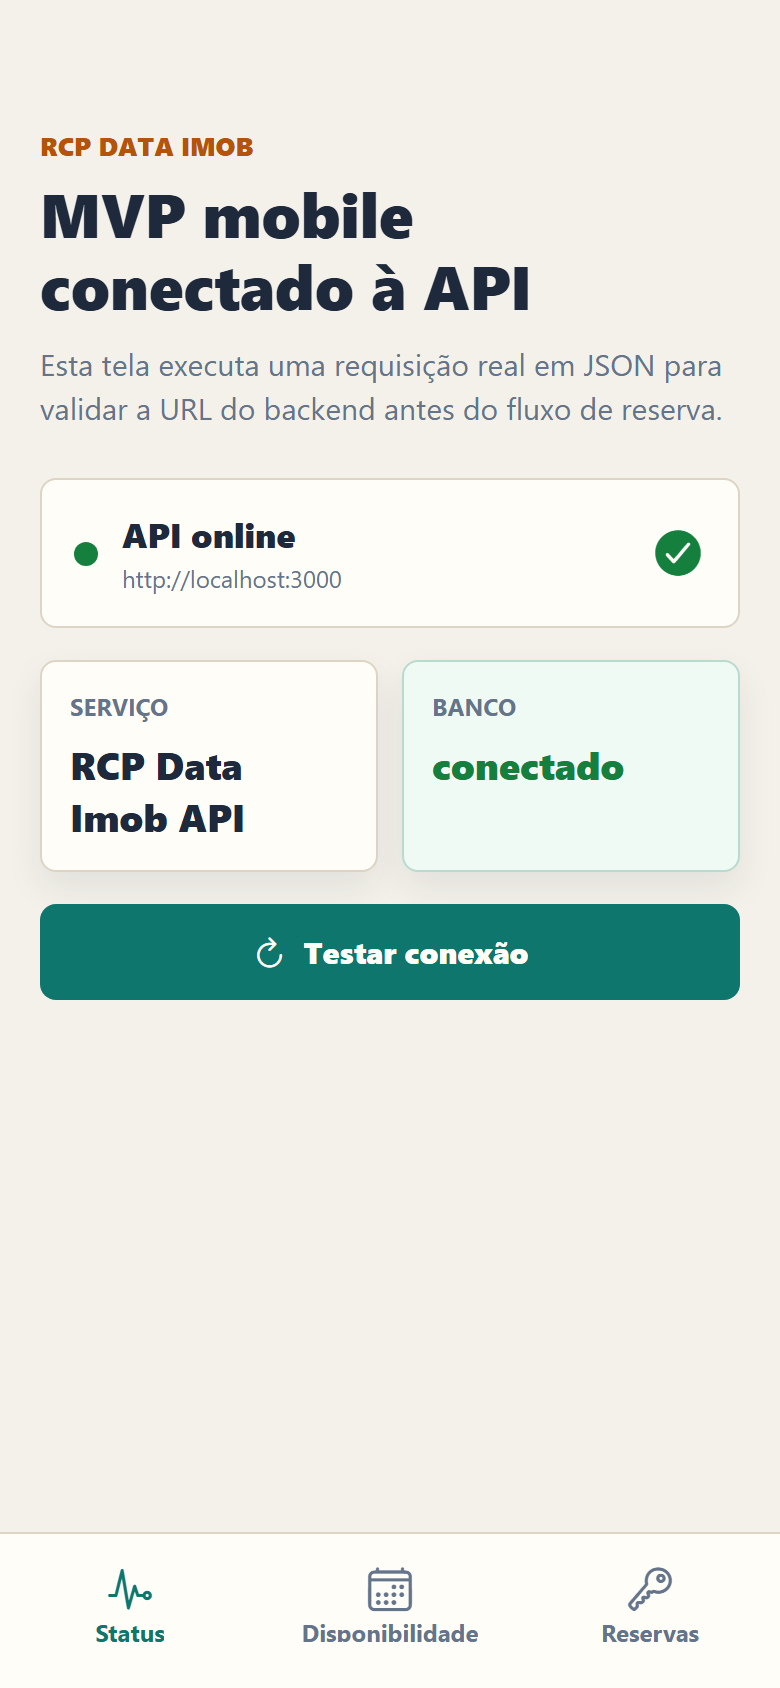
\includegraphics[width=0.31\textwidth]{screenshots/mobile/mobile-status-api.png}
  \hfill
  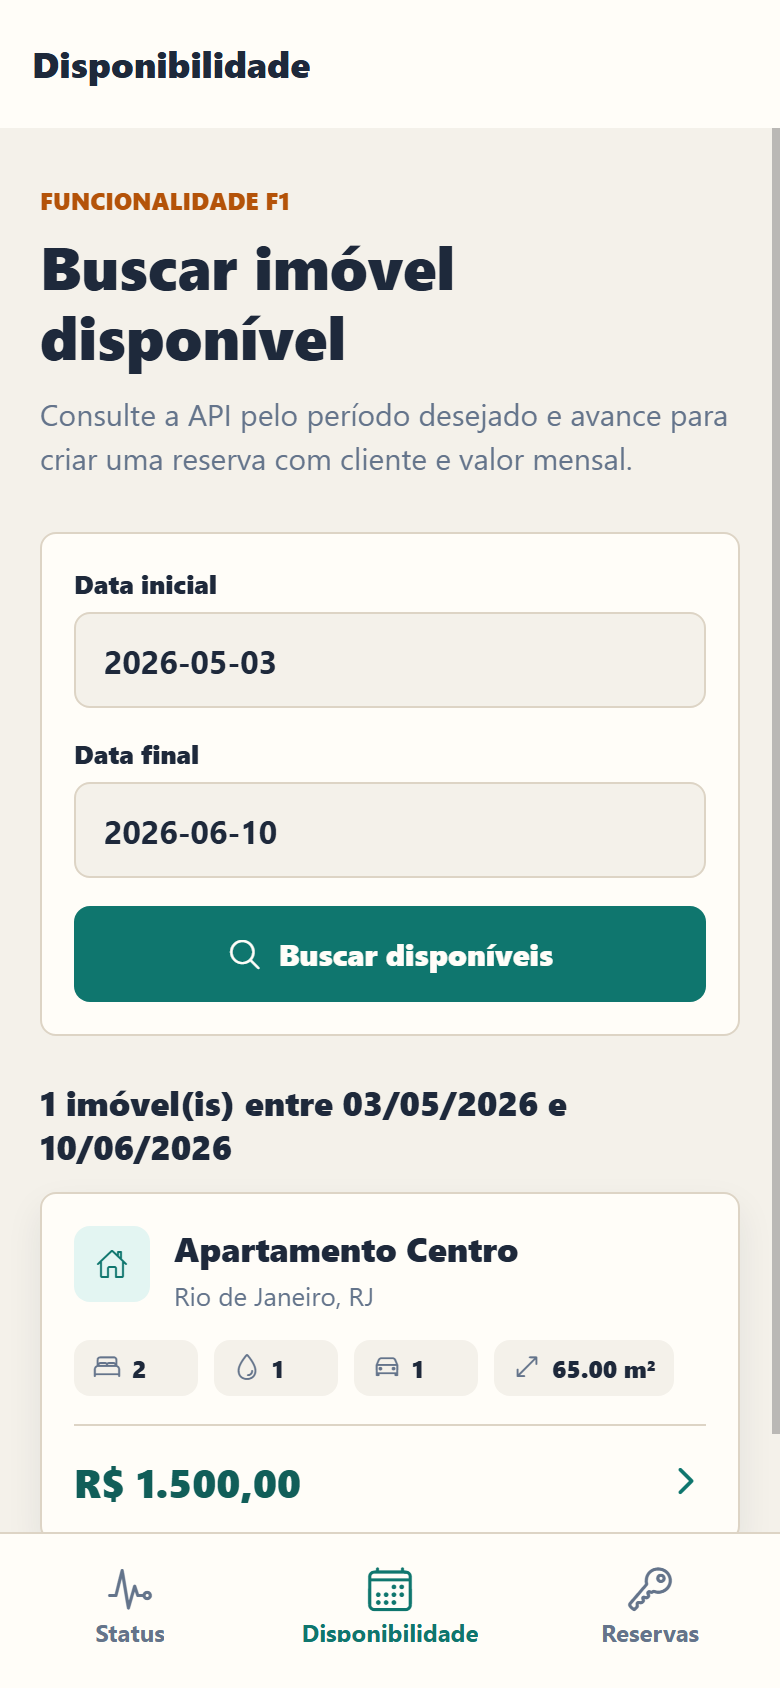
\includegraphics[width=0.31\textwidth]{screenshots/mobile/mobile-disponibilidade.png}
  \hfill
  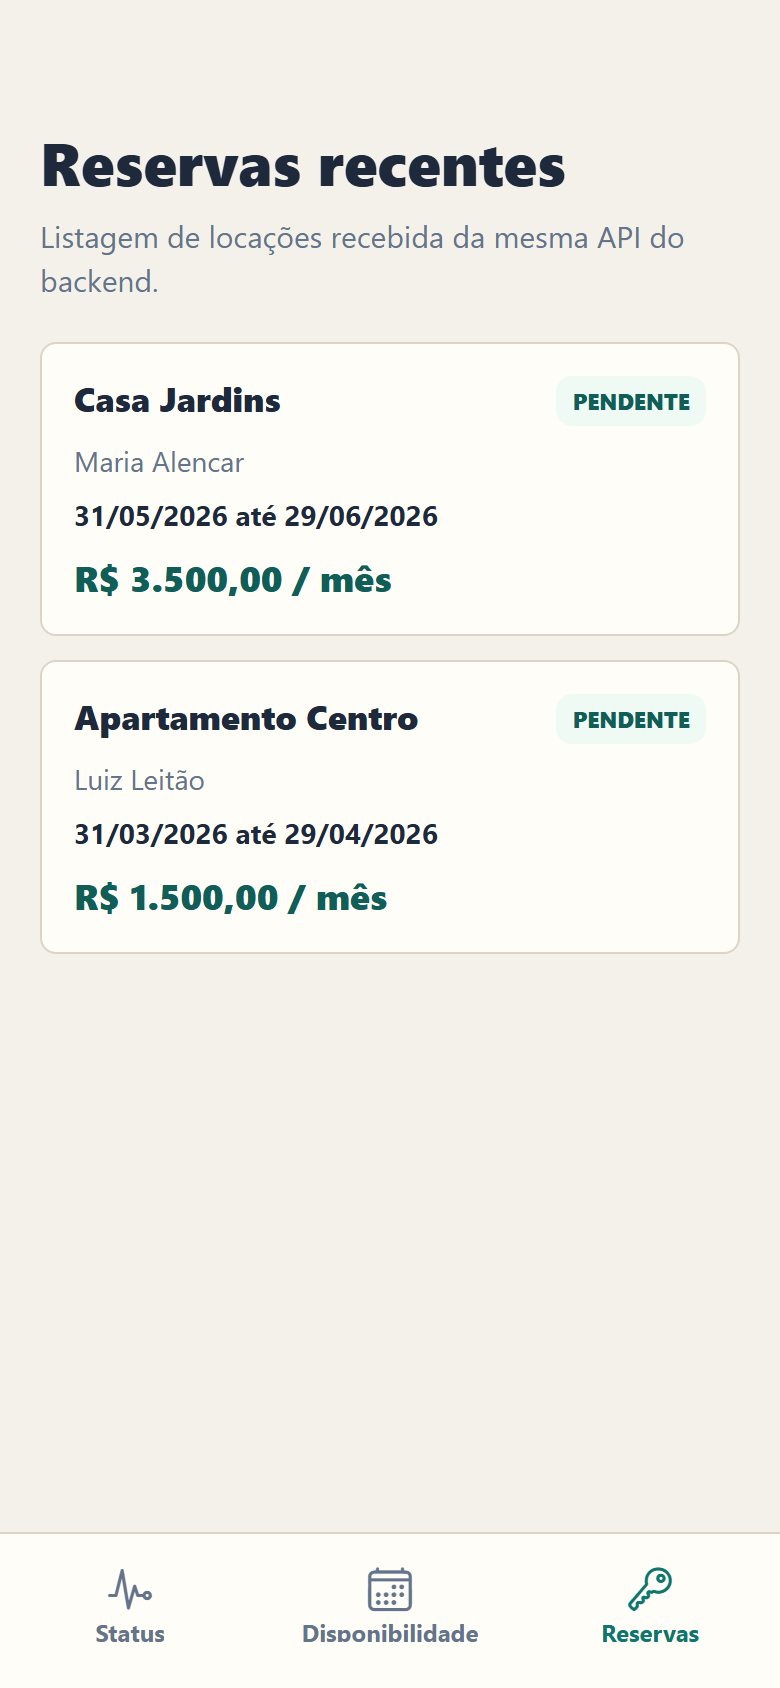
\includegraphics[width=0.31\textwidth]{screenshots/mobile/mobile-reservas.png}
  \caption{Telas mobile: status da API, busca de disponibilidade e reservas recentes}
  \label{fig:mobile-mvp}
\end{figure}

% ══════════════════════════════════════════════════════════════════════════════
\section{Execução do Ambiente}

O projeto foi preparado para execução com Docker Compose, permitindo subir todos os serviços de forma integrada.

\begin{lstlisting}
# Subir todos os servicos (build + start em background)
docker compose up --build -d

# Verificar status dos containers
docker compose ps

# Ver logs de um servico especifico
docker compose logs frontend
docker compose logs backend

# Parar os servicos
docker compose down

# Remover tambem os volumes (apaga dados do banco)
docker compose down -v
\end{lstlisting}

Para executar o app mobile com Expo:

\begin{lstlisting}
cd mobile
npm install
npm start
\end{lstlisting}

\subsection{Acessos}

\begin{table}[H]
\centering
\begin{tabular}{|l|l|}
\hline
\thead{Serviço} & \thead{URL} \\
\hline
Frontend    & http://localhost:5173 \\
\talt API REST    & http://localhost:3000 \\
PostgreSQL  & localhost:5432 \\
\talt Mobile Expo & Expo Go / emulador via \texttt{npm start} em \texttt{mobile/} \\
\hline
\end{tabular}
\caption{URLs de acesso aos serviços}
\end{table}

\subsection{Telas Disponíveis}

\begin{table}[H]
\centering
\begin{tabularx}{\textwidth}{|l|X|}
\hline
\thead{Rota} & \thead{Tela} \\
\hline
/                & Dashboard — KPIs e gráfico financeiro \\
\talt /imoveis        & Gestão de Imóveis \\
/clientes        & Gestão de Clientes \\
\talt /locacoes       & Gestão de Locações (com status F2) \\
/financeiro      & Controle Financeiro \\
\talt /disponibilidade & Busca de Disponibilidade e Reserva (F1) \\
/calendario      & Agenda Mensal com Calendário (F2) \\
\hline
\end{tabularx}
\caption{Telas disponíveis no sistema}
\end{table}

\subsection{Telas Mobile Disponíveis}

\begin{table}[H]
\centering
\begin{tabularx}{\textwidth}{|l|X|}
\hline
\thead{Aba / Tela} & \thead{Função} \\
\hline
Status & Validação da API com \texttt{GET /status} \\
\talt Disponibilidade & Fluxo F1: busca de imóveis, detalhe e reserva \\
Reservas & Consulta das locações registradas \\
\hline
\end{tabularx}
\caption{Telas disponíveis no MVP mobile}
\end{table}

% ══════════════════════════════════════════════════════════════════════════════
\section{Considerações sobre a Implementação}

A proposta do sistema demonstra uma evolução consistente ao longo dos entregáveis:

\begin{itemize}[leftmargin=1.5em]
  \item No \textbf{Entregável 0}, foi definida a proposta do sistema, seu escopo funcional, a stack e a visão geral das telas;
  \item No \textbf{Entregável 2}, foi consolidada a implementação da API REST, com organização modular, integração com PostgreSQL e endpoints CRUD por entidade;
  \item No \textbf{Entregável 3}, foi configurado o banco de dados PostgreSQL via Docker, com modelagem completa das entidades, inicialização automática do schema e validação de CRUD via Postman;
  \item No \textbf{Entregável 4}, foi implementado o frontend completo com React, Vite e Tailwind CSS, configurado no Docker com proxy para o backend, consumindo dados reais da API em todas as 5 telas do sistema;
  \item No \textbf{Entregável 5}, foi implementada a Funcionalidade F1 completa (Busca de Disponibilidade e Criação de Reserva), com novo endpoint de API com lógica de conflito de datas, nova tela no frontend e fluxo de reserva end-to-end funcionando no Docker;
  \item No \textbf{Entregável 6}, foi implementada a Funcionalidade F2 completa (Sistema de Reservas com Status), com ciclo de vida completo de reservas, calendário mensal interativo, cálculo automático de valor total e edição com revalidação de conflito;
  \item No \textbf{Entregável 7}, foi implementada a Funcionalidade F3 completa (Controle Financeiro com Dashboard Analítico), com endpoints de agregação no backend, filtros avançados, edição e exclusão de lançamentos, marcação automática de atrasados, gráfico de pizza por status e Dashboard alimentado por SQL agregado;
  \item No \textbf{Entregável 8}, foi criado o MVP mobile com React Native e Expo, consumindo a mesma API do backend e implementando o fluxo principal da F1 em navegação mobile.
\end{itemize}

% ══════════════════════════════════════════════════════════════════════════════
\section{Conclusão}

O Sistema de Gestão de Locações de Imóveis (RCP Data Imob) foi projetado e implementado como uma solução web completa para atender às necessidades de uma administradora de imóveis. O sistema integra cadastro, locações, categorização e controle financeiro em uma única aplicação com interface visual profissional.

Do ponto de vista técnico, a solução utiliza tecnologias atuais e amplamente adotadas no desenvolvimento web, com separação clara entre frontend, backend e banco de dados. A utilização de Docker Compose contribui para a reprodutibilidade do ambiente, enquanto a API REST organizada por entidade favorece escalabilidade e manutenção.

O frontend implementado oferece uma experiência de usuário completa, com Dashboard analítico, CRUD funcional em todas as entidades, design responsivo com Tailwind CSS, gráficos interativos com Recharts, e micro-interações que conferem profissionalismo à interface.

O Entregável 6 finaliza a Funcionalidade F2, completando o ciclo de vida das reservas com controle de status, calendário mensal de ocupações, cálculo automático de valor total e validação rigorosa de conflitos de datas.

O Entregável 7 conclui o terceiro pilar do escopo, entregando a Funcionalidade F3 (Controle Financeiro com Dashboard Analítico). A API ganhou endpoints de agregação (\texttt{/financeiro/resumo} e \texttt{/financeiro/por-mes}), além de filtros, edição (PUT), exclusão (DELETE) e marcação automática de lançamentos vencidos como atrasados. A tela de Financeiro foi reescrita com 4 KPIs, gráfico de pizza por status, filtros expandidos e CRUD completo via modal. O Dashboard agora consome a agregação direto do SQL, eliminando processamento no cliente. Com isso, todos os três módulos do escopo (F1, F2 e F3) estão operando ponta-a-ponta no ambiente Docker.

O Entregável 8 amplia a solução para o ambiente mobile. O app React Native criado em \texttt{mobile/} possui navegação por abas, tela de status da API, busca de disponibilidade, detalhe do imóvel, confirmação de reserva e listagem de locações. O fluxo consome os mesmos endpoints do backend, com URL configurável para computador na rede local, mantendo a API como ponto único de integração entre web e mobile.

% ══════════════════════════════════════════════════════════════════════════════
\section{Referências Internas do Projeto}

\begin{itemize}[leftmargin=1.5em]
  \item Entregável 0 — Definição do tema, escopo, stack e telas;
  \item Entregável 2 — Implementação da API REST e organização do backend;
  \item Entregável 3 — Banco de dados PostgreSQL + Docker + testes CRUD via Postman;
  \item Entregável 4 — Frontend React + Vite + Tailwind CSS no Docker, consumindo API;
  \item Entregável 5 — Funcionalidade F1: Busca de Disponibilidade e Criação de Reserva;
  \item Entregável 6 — Funcionalidade F2: Sistema de Reservas com Status e Calendário Mensal;
  \item Entregável 7 — Funcionalidade F3: Controle Financeiro com Dashboard Analítico;
  \item Entregável 8 — MVP mobile React Native: F1 no app mobile consumindo a API;
  \item Coleção Postman — \texttt{postman/RCP\_Data\_Imob.postman\_collection.json}.
\end{itemize}

\vspace{2cm}
\begin{center}
  \color{gray60}\rule{0.5\textwidth}{0.4pt}\\[8pt]
  {\small Marcell Parra Araújo B. Silva \quad•\quad Rafael Vargas Carvalheira \quad•\quad Ruan Pablo Rodrigues}\\[4pt]
  {\small\color{teal} Março de 2026 — atualizado em Maio de 2026 (Entregável 8)}
\end{center}

\end{document}
